\documentclass[tikz,border=3pt]{standalone}
\usepackage[utf8]{inputenc}
\usepackage[T1]{fontenc}
\usepackage{lmodern}
\renewcommand{\familydefault}{\sfdefault}
\usepackage{sansmath}\sansmath
\usepackage{chemfig}
\usepackage{pgfplots}\pgfplotsset{compat=1.18,/pgf/number format/use comma,/pgf/number format/1000 sep={.}}
\usetikzlibrary{arrows.meta,calc,positioning,decorations.pathmorphing,patterns}
% paleta del sitio
\definecolor{nar}{HTML}{E8680C}\definecolor{narc}{HTML}{FFB35C}\definecolor{hielo}{HTML}{FFF3E8}
\definecolor{tinta}{HTML}{1D1D1F}\definecolor{gris}{HTML}{6E6E73}\definecolor{lila}{HTML}{7C5CF0}
\definecolor{azul}{HTML}{2F6FD6}\definecolor{menta}{HTML}{17A673}\definecolor{coral}{HTML}{E8342A}
\begin{document}
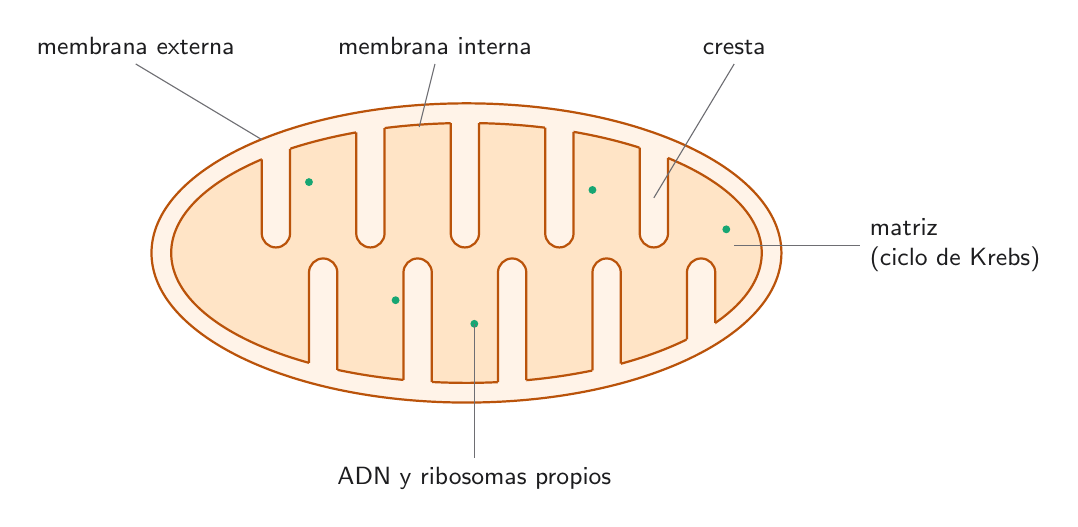
\begin{tikzpicture}[font=\small]
\draw[nar!80!black,thick,fill=hielo] (0,0) ellipse (4.0 and 1.9);
\draw[nar!80!black,thick,fill=narc!35] (0,0) ellipse (3.75 and 1.65);
\fill[hielo] (-2.60,1.249) -- (-2.60,0.25) arc (180:360:0.18) -- (-2.24,1.383) -- cycle;
\draw[nar!80!black,thick] (-2.60,1.189) -- (-2.60,0.25) arc (180:360:0.18) -- (-2.24,1.323);
\fill[hielo] (-1.40,1.591) -- (-1.40,0.25) arc (180:360:0.18) -- (-1.04,1.645) -- cycle;
\draw[nar!80!black,thick] (-1.40,1.531) -- (-1.40,0.25) arc (180:360:0.18) -- (-1.04,1.585);
\fill[hielo] (-0.20,1.708) -- (-0.20,0.25) arc (180:360:0.18) -- (0.16,1.708) -- cycle;
\draw[nar!80!black,thick] (-0.20,1.648) -- (-0.20,0.25) arc (180:360:0.18) -- (0.16,1.648);
\fill[hielo] (1.00,1.650) -- (1.00,0.25) arc (180:360:0.18) -- (1.36,1.598) -- cycle;
\draw[nar!80!black,thick] (1.00,1.590) -- (1.00,0.25) arc (180:360:0.18) -- (1.36,1.538);
\fill[hielo] (2.20,1.396) -- (2.20,0.25) arc (180:360:0.18) -- (2.56,1.266) -- cycle;
\draw[nar!80!black,thick] (2.20,1.336) -- (2.20,0.25) arc (180:360:0.18) -- (2.56,1.206);
\fill[hielo] (-2.00,-1.456) -- (-2.00,-0.25) arc (180:0:0.18) -- (-1.64,-1.544) -- cycle;
\draw[nar!80!black,thick] (-2.00,-1.396) -- (-2.00,-0.25) arc (180:0:0.18) -- (-1.64,-1.484);
\fill[hielo] (-0.80,-1.672) -- (-0.80,-0.25) arc (180:0:0.18) -- (-0.44,-1.699) -- cycle;
\draw[nar!80!black,thick] (-0.80,-1.612) -- (-0.80,-0.25) arc (180:0:0.18) -- (-0.44,-1.639);
\fill[hielo] (0.40,-1.701) -- (0.40,-0.25) arc (180:0:0.18) -- (0.76,-1.676) -- cycle;
\draw[nar!80!black,thick] (0.40,-1.641) -- (0.40,-0.25) arc (180:0:0.18) -- (0.76,-1.616);
\fill[hielo] (1.60,-1.552) -- (1.60,-0.25) arc (180:0:0.18) -- (1.96,-1.467) -- cycle;
\draw[nar!80!black,thick] (1.60,-1.492) -- (1.60,-0.25) arc (180:0:0.18) -- (1.96,-1.407);
\fill[hielo] (2.80,-1.158) -- (2.80,-0.25) arc (180:0:0.18) -- (3.16,-0.948) -- cycle;
\draw[nar!80!black,thick] (2.80,-1.098) -- (2.80,-0.25) arc (180:0:0.18) -- (3.16,-0.888);
\foreach \p in {(-2.0,0.9),(0.1,-0.9),(1.6,0.8),(-0.9,-0.6),(3.3,0.3)} \fill[menta] \p circle (0.05);
\draw[gris] (-2.6,1.44) -- (-4.2,2.4) node[anchor=south,text=tinta] {membrana externa};
\draw[gris] (-0.6,1.6) -- (-0.4,2.4) node[anchor=south,text=tinta] {membrana interna};
\draw[gris] (2.38,0.7) -- (3.4,2.4) node[anchor=south,text=tinta] {cresta};
\draw[gris] (3.4,0.1) -- (5.0,0.1) node[anchor=west,text=tinta,align=left] {matriz\\(ciclo de Krebs)};
\draw[gris] (0.1,-0.9) -- (0.1,-2.6) node[anchor=north,text=tinta] {ADN y ribosomas propios};
\end{tikzpicture}
\end{document}
